\section{Le 6 W}

Analizziamo ora i 6 assi partendo dall'homepage. Un sito ben progettato è in grado di 
dare all'utente l'informazione o gli strumenti necessari per poter ricavare queste informazioni
il più velocemente possibile dal sito. Vediamo i sei assi nel dettaglio, sia per quanto riguarda
l'homepage, che, in caso di necessità, per una pagina a caso del sito (la pagina del 
\emph{Guerriero}, nel nostro caso). 

\subsection{Who?}
\begin{quote}
    \emph{``Chi rappresenta il sito?''}
\end{quote}
Per rispondere a quest'asse, è sufficiente guardare il logo dall'\emph{header} della homepage o di 
una qualsiasi pagina interna.
\begin{figure}[hbt]
    \centering
    
\includegraphics[width=5cm]{img/logo.png}
    \caption{Logo del sito Golarion Insider.}
\end{figure}

Il nome del sito, \textbf{Golarion Insider}, è scritto in un font non troppo distinguibile e accompagnato da uno sfondo 
con colori che rischiano di confondersi con quello usato per le parole. Almeno, è stata scelta la miglior posizione per un logo.
C'è inoltre da notare che l'header occupa forse troppo spazio, rischiando di portare l'utente che usa schermi di piccole dimensioni
a scrollare per vedere del contenuto
(soprattutto per la versione mobile del sito, di cui parleremo in seguito).

\subsection{What?}
\begin{quote}
    \emph{``Cosa offre il sito?''}
\end{quote}

L'utente che si ritroverà nella homepage, andrà generalmente a cliccare sulla sezione del menù che gli interessa (\emph{Caratteristiche, %
Talenti, Classi,} etc\dots), per ritrovarsi catapultato nella pagina interna di suo interesse. Il sito offre esattamente quello
per cui è nato: un database con tutte le informazioni riguardanti il mondo di gioco di \textbf{Pathfinder}.

\newpage
Diamo un'occhiata a una pagina interna: quella del \href{http://golarion.altervista.org/wiki/Guerriero}{Guerriero}.

\begin{figure}[hbt]
    \centering
    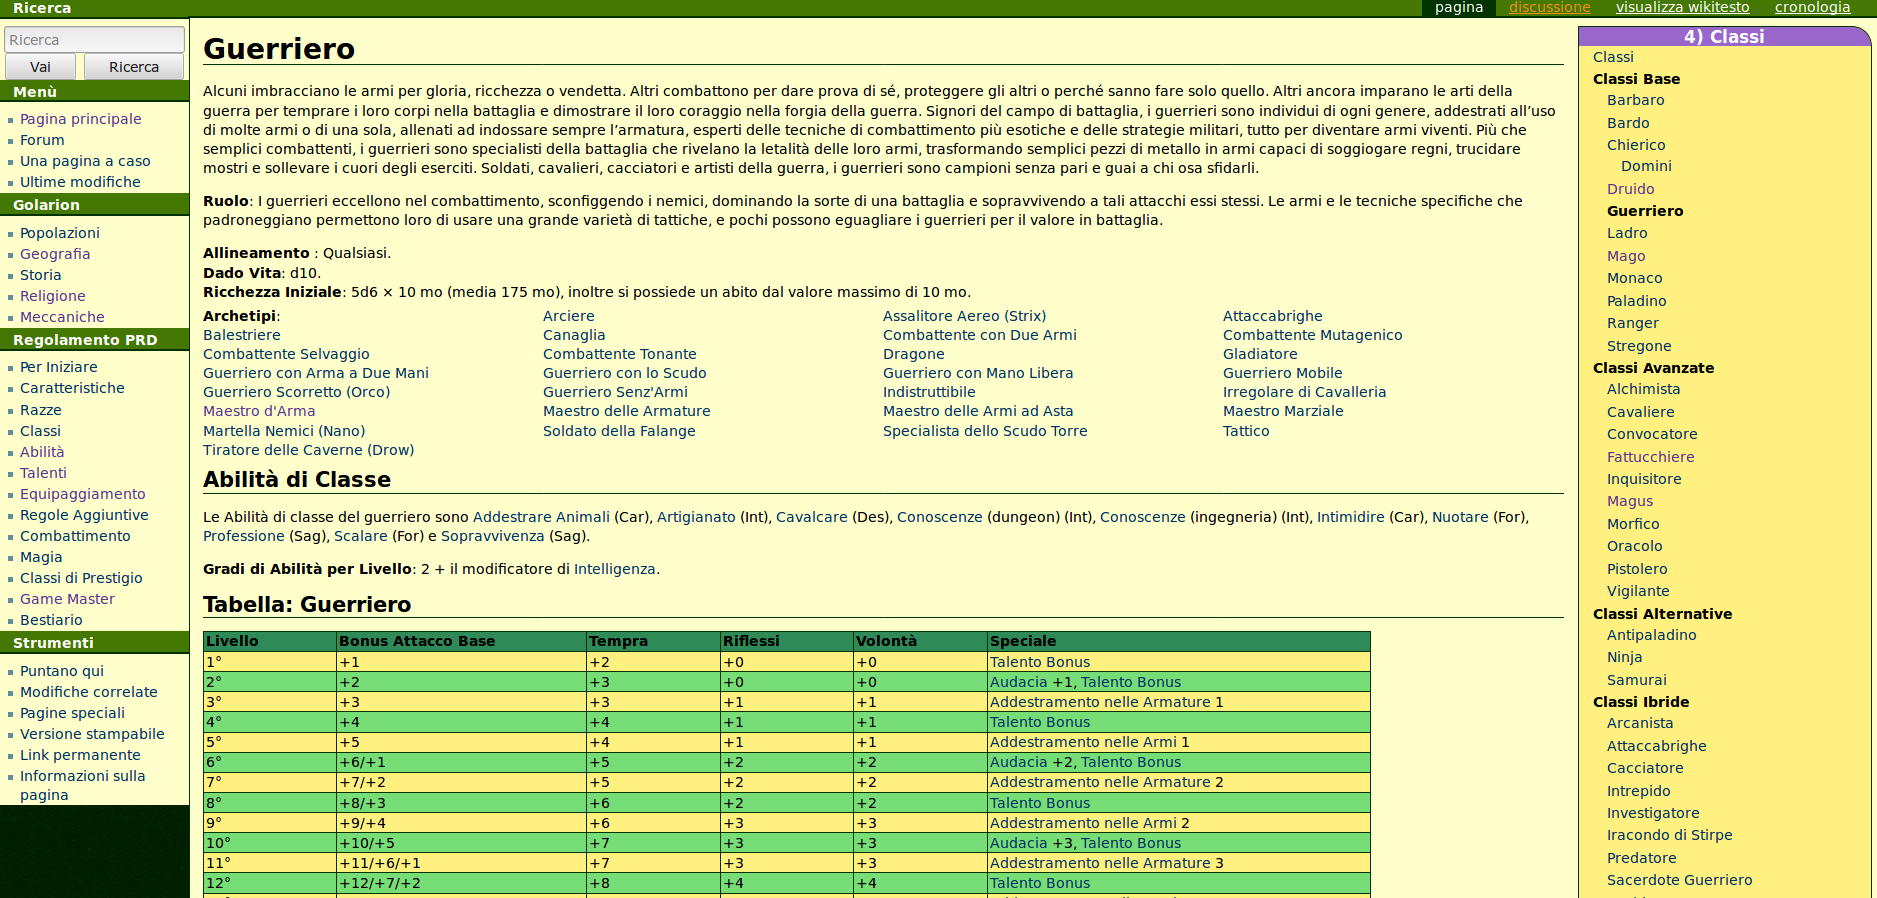
\includegraphics[width=\textwidth]{img/guerriero.png}
    \caption{Pagina relativa alla classe del Guerriero.}
    \label{fig:guerriero}
\end{figure}

In questa pagina sono raccolte tutte le regole relative al Guerriero, che è quello che l'utente, giunto a questa pagina tramite un link, si aspetta.
A sinistra è presente il menù, a destra una raccolta di tutte le classi suddivise per tipo, e in alto l'header (omesso nell'immagine) 
con un link alla homepage.\par
In base alla quantità di informazioni necessarie per l'argomento specifico, possono essere necessari anche 3 o più
scroll per leggere tutto. Ciò risulta comunque inevitabile per l'obiettivo prefissato dal sito.

\clearpage

\subsection{When?}
\begin{quote}
    \emph{``Quali sono le ultime novità? Quando è stato mantenuto per l'ultima volta?''}
\end{quote}

Nel \emph{footer} di ogni pagina, è presente una stringa generata da uno script che riporta quando la pagina è stata 
modificata per l'ultima volta (e.g., nella homepage: ``Questa pagina è stata modificata per l'ultima volta il 27 gen 2018 alle 15:40.'').

Oltre a questo, essendo una \texttt{wiki} e rispettando i canoni di questo media, è possibile visionare \emph{tutte} le
\href{http://golarion.altervista.org/api.php?hidebots=1&days=7&limit=50&hidecategorization=1&action=feedrecentchanges&feedformat=atom}{modifiche}
che sono state effettuate al sito, dagli utenti, tramite il primo bottone presente sotto al logo: 

\begin{figure}[hbt]
    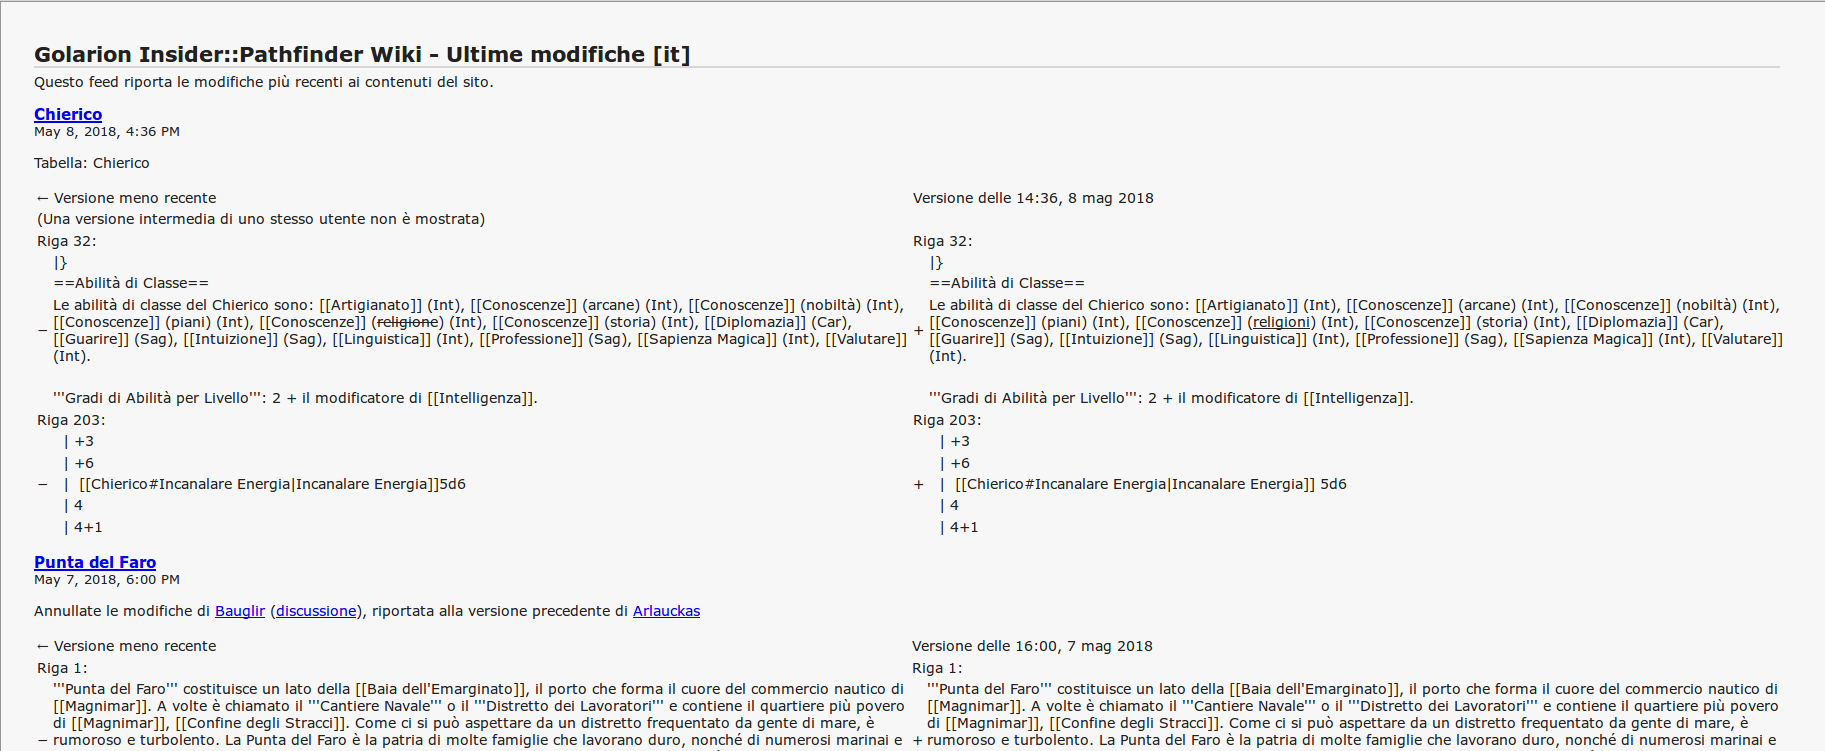
\includegraphics[width=\textwidth]{img/ultime_modifiche.png}
    \caption{Ultime modifiche effettuate dagli utenti.}
\end{figure}

\subsection{Why?}
\begin{quote}
    \emph{``Perchè mai dovrei fermarmi su questo sito? Quali benefici mi porta?''}
\end{quote}

Golarion Insider, come già fatto notare in precedenza, è un sito riservato ai visitatori interessati a documentarsi sul
gioco di ruolo in questione. Difficilmente, anzi, per nessun motivo, qualsiasi altro utente si recherebbe in questo sito, e
se anche lo facesse, se ne andrebbe dopo aver capito di cosa si tratta, per ovvie ragioni.

\subsection{How?}
\begin{quote}
    \emph{``Come faccio ad arrivare alle sezioni principali?''}
\end{quote}
Come già anticipato nella sezione \ref{analisipre}, la navigazione si limita a un menù laterale in cui raggiungere le sezioni,
ed è difficile stabilire una vera gerarchia del sito.

\subsection{Where?}
\begin{quote}
    \emph{``A che tipo di sito sono arrivato? Come sono posizionato all'interno della gerarchia?''}
\end{quote}

Qui iniziano le vere note dolenti. Raggiunta una qualsiasi pagina del sito, non si ha alcuna informazione sulla posizione
all'interno della gerarchia del sito; il problema è alimentato dal fatto che la maggior parte delle visite avviene tramite
\emph{deep linking}. Non è presente alcuna forma di \textbf{breadcrumb}, come visibile nella pagina (ad esempio) del Guerriero 
(figura \ref{fig:guerriero}).
Il menù a destra è relativo ad ogni ``sezione'' (ad esempio, per le \emph{Classi} o per i \emph{Talenti}), e sembra l'unico modo 
per farsi un'idea sulla posizione in cui si è in un dato momento. Vengono utilizzati link con colori standard: blu per gli unvisited, viola 
per i visited. \par
La navigazione, personalmente, è risultata spesso confusa per le ragioni sopracitate.